\documentclass[11pt,a4paper]{article}
\usepackage[utf8]{inputenc}
\usepackage{tikz}
\usetikzlibrary{decorations.pathreplacing}
\usepackage{microtype}
\usepackage{amsmath}
\usepackage{amsfonts}
\usepackage{amssymb}
\usepackage{xargs}
\usepackage[parfill]{parskip}
\usepackage[margin=1.3in]{geometry}
\usepackage{tabularx}
\usepackage{float}
\usepackage{amsthm}

%\usepackage{ccfonts}
%\usepackage[adobe-utopia]{mathdesign}
%\usepackage{eucal}
%\usepackage{arev}
%\usepackage[T1]{fontenc}
%\usepackage{fontspec}
%\setmainfont{Asana-Math}
%\usepackage[adobe-utopia]{mathdesign}
\usepackage{libertinus}
\usepackage{fdsymbol}
\usepackage[T1]{fontenc}


\usepackage[ruled,vlined,linesnumbered,noend]{algorithm2e}
\usepackage{setspace}

%\def\arraystretch{1.2}

\newcommand{\Qc}{\mathcal{Q}}
\newcommand{\Sc}{\mathcal{S}}
\newcommand{\E}{\mathbb{E}}
\newcommand{\Act}{\mathrm{Act}}
\newcommand{\Ac}{\mathcal{A}}
\newcommand{\dt}{\matrm{\ d}}
\newcommand{\KL}{\mathrm{KL}}
\newcommand{\Af}{\mathbf{A}}
\newcommand{\bfat}{\mathbf{b}}
\newcommand{\xf}{\mathbf{x}}
\newcommand{\af}{\mathbf{a}}
\newcommand{\yf}{\mathbf{y}}
\newcommand{\Df}{\mathbf{D}}
\newcommand{\cf}{\mathbf{c}}
\newcommand{\ef}{\mathbf{e}}
\newcommand{\gf}{\mathbf{g}}
\newcommand{\df}{\mathbf{d}}
\newcommand{\Lc}{\mathcal{L}}
\newcommand{\Uc}{\mathcal{U}}
\newcommand{\Be}{\mathrm{Be}}
\newcommand{\Mult}{\mathrm{Mult}}
\newcommand{\Nc}{\mathcal{N}}
\newcommand{\Fc}{\mathcal{F}}
\newcommand{\R}{\mathbb{R}}
\newcommand{\N}{\mathbb{N}}
\newcommand{\Cov}{\mathrm{Cov}}
\newcommand{\Var}{\mathrm{Var}}
\newcommand{\dom}{\mathrm{dom}}
\newcommand{\st}{\text{subject to}}

\DeclareMathOperator*{\argmax}{\arg\max}
\DeclareMathOperator*{\argmin}{\arg\min}
\newcommand{\pdata}{p_\mathrm{data}}
\newcommand{\pmodel}{p_\mathrm{model}}
\numberwithin{equation}{section}


\newcommand{\idx}{\varphi}
\newcommand{\varidx}{\psi}
\newcommand{\move}[3]{#1_{#2\rightarrow #3}}
\newcommand{\image}{\mathrm{image}}
\newcommand{\minimize}{\text{minimize}}
\renewcommand{\iff}{\quad\text{iff}\quad}

% \newtheoremrep{theorem}{Theorem}[section]
% \newtheoremrep{corollary}{Corollary}[theorem]
% \newtheoremrep{lemma}[theorem]{Lemma}
\newtheorem{definition}{Definition}[section]

% \usepackage{apxproof}
\newtheorem{theorem}{Theorem}[section]
\newtheorem{corollary}{Corollary}[theorem]
\newtheorem{lemma}[theorem]{Lemma}
\newtheorem{theoremrep}{Theorem}[section]
\newtheorem{corollaryrep}{Corollary}[theorem]
\newtheorem{lemmarep}[theorem]{Lemma}
\newcommand{\appendixproof}{proof}

\begin{document}

\tableofcontents
\newpage

% Problem with multicuts: they require a lot of store, since they are bounded by |V|^2.
% Thus, focus on partition-perspective on problem.
% Problem with partitions in set-format: hard to check equalities between partitions set-format and transformations require set-operations that might take a lot of time.
% Therefore: introduce indexings

\section{Notation}
Let $A$ be some set. We will denote the set $\{ \{ a_1, \dots, a_k \} \subseteq A : a_1,\dots,a_k\ \text{pairwise distinct}\}$, which contains all $k$-ary subsets of $A$, by $\binom{A}{k}$. For the same set $A$, $P_A$ denotes the set of all partitions of $A$. For a partition $\Pi \in P_A$ and an element $a \in A$, $[a]_\Pi$ denotes the set in $\Pi$ that contains $a$, of which there is exactly one. If $A$ is finite, $\Uc(A)$ denotes the uniform distribution over $A$, i.e. the distribution that assigns every element in $A$ the same probability (namely: $1/|A|$). If we want to indicate that a random variable ${\bf X}$ has probability distribution $\mathcal{Q}$, we will write ${\bf X} \sim \mathcal{Q}$. If $f$ is a function from the domain of a random variable ${\bf X} \sim \mathcal{Q}$ to the real numbers, its expected value is written as $\E_{{\bf X} \sim \mathcal{Q}}\left[f({\bf X})\right]$.  

\section{Introduction}
Let $V = \{ v_1,\dots,v_n \}$ be a finite set of vertices. Associated with this set are functions $c,c': \binom{V}{3} \mapsto \R$ which define cost-structures on $3$-ary subsets of $V$. For a $3$-ary subset $\{u,v,w\} \in \binom{V}{3}$ and a given partition $\Pi \in P_V$, we define the cost of $\{u,v,w\}$ with respect to $\Pi$ as  
\begin{align*}
    \ell(\{u,v,w\},\Pi) = \begin{cases}
        c(\{u,v,w\}) & \text{if}\ [u]_\Pi \neq [v]_\Pi, [u]_\Pi \neq [w]_\Pi, [w]_\Pi \neq [v]_\Pi \\
        c'(\{u,v,w\}) & \text{if}\ [u]_\Pi = [v]_\Pi = [w]_\Pi \\
        0 & \text{otherwise.}
    \end{cases}
\end{align*}
This can be interpreted as follows: whenever $u,v$ and $w$ are part of pairwise different sets in $\Pi$, the cost of $\{u,v,w\}$ is equal to the costs as defined by $c$. If they are part of the same set, the cost of $\{u,v,w\}$ is equal to the costs as defined by $c'$. Otherwise, if neither of the above is the case, the cost of $\{u,v,w\}$ is just $0$. Based on this definition, we are confronted with problems of the form
\begin{align*}
    \Pi^* = \argmin_{\Pi \in P_V} \sum\nolimits_{\{u,v,w\} \in \binom{V}{3}} \ell(\{u,v,w\},\Pi)
\end{align*}
i.e. we wish to find a partition $\Pi^*$ of $V$ that minimizes some objective function over $3$-ary subsets of $V$. This problem is hard in many respects: one, the amount of possible partitions grows large very fast (with growing $n$). Two, even computing the objective function for a given partition is prohibitive, since summing over all $3$-ary subsets takes almost $n^3$ steps (and to add to that, not even $n^2$ steps are feasible if $n$ becomes larger). Thus, we are interested in a way of approximately solving this problem by the use of a local search algorithm and some considerations on the objective function.

\paragraph{Approximizing the Objective Function}
Since we are only interested in some minimizer $\Pi^*$ of the above problem, it does not matter which function we minimize, as long as the set of minimizers stays the same. Therefore, we can apply any strongly monotonic growing function to the objective, and, for example, multiply by some constant. We are then able to obtain
\begin{align*}
    \Pi^* &= \argmin_{\Pi \in P_V} \sum\nolimits_{T\in\binom{V}{3}} \ell(T,\Pi) \\
    &= \argmin_{\Pi \in P_V} \frac{1}{|\binom{V}{3}|} \sum\nolimits_{T\in\binom{V}{3}} \ell(T,\Pi) \\
    &= \argmin_{\Pi \in P_V} \mathbb{E}_{{\bf T} \sim \Uc\left(\binom{V}{3}\right)} \left[\ell({\bf T}, \Pi)\right]
\end{align*}
where $\Uc(\binom{V}{3})$ is the uniform distribution over $\binom{V}{3}$. This perspective allows to approximate the objective value to any degree by uniformly sampling a fixed number of $3$-ary subsets from $V$ and then computing the sample mean. In many cases, one wants to compute the change in the objective function when considering two different partitions $\Pi,\Pi' \in P_V$. The difference is then given by
\begin{align*}
    \mathbb{E}_{{\bf T} \sim \Uc\left(\binom{V}{3}\right)} \left[\ell({\bf T}, \Pi)\right] - \mathbb{E}_{{\bf T} \sim \Uc\left(\binom{V}{3}\right)} \left[\ell({\bf T}, \Pi')\right] = \mathbb{E}_{{\bf T} \sim \Uc\left(\binom{V}{3}\right)} \left[\ell({\bf T}, \Pi) - \ell({\bf T}, \Pi')\right],
\end{align*}
which can possibly be simplified, dependent on the shape of $\Pi'$ with respect to $\Pi$ and vice versa.
\section{Indexings as Proxies for Partitions}
Since we want to use a local search algorithm that iteratively finds better solutions (partitions in this case), the second consideration is on how we want to represent said partitions. One may represent a partition as a set of sets of vertices, which is probably the most straight-forward approach. On the one hand, the required space is linear in $n$. But on the other hand, this comes with a few problems: checking if two vertices are part of the same set, and the removal and the addition of a vertex from or to a set all require $n$ steps in the worst case (if all vertices have the same set). A last problem is that one has to gurantee consistency at every step, i.e. that every solution is indeed a partition. A second idea might be to store a partition as a $n \times n$ boolean matrix, where every row corresponds to a vertex and every column to a set in the partition, and an entry at position $i,j$ would mean ``vertex $i$ is part of set $j$'' if $1$ and ``vertex $i$ is not part of set $j$'' if $0$. This would alleviate some of the above problems, since looking up, removal or addition of vertices to sets would take constant time in the worst case. However, storing a partition would require $n^2$ units of space, which might become problematic when $n$ is large or when considering multiple partitions at once.

Therefore, we will use the following concept of indexings (which are similar to equivalence relations) to solve the above problems, i.e. to simplify and speed up operations on partitions. Every vertex is mapped to a number (index) which indicates the set in the partition we want this vertex to be a part of. If multiple vertices are mapped to the same index, they will be part of the same set in the partition. Since there are at maximum $n$ sets in a partition of $V$ (every vertex is assigned its own set, i.e. the indexing is bijective), we restrict to indices between $1$ and $n$. Note that every indexing can be stored in a linear amount of memory dependent on the size of $V$.


\begin{figure}[ht]
    \centering
    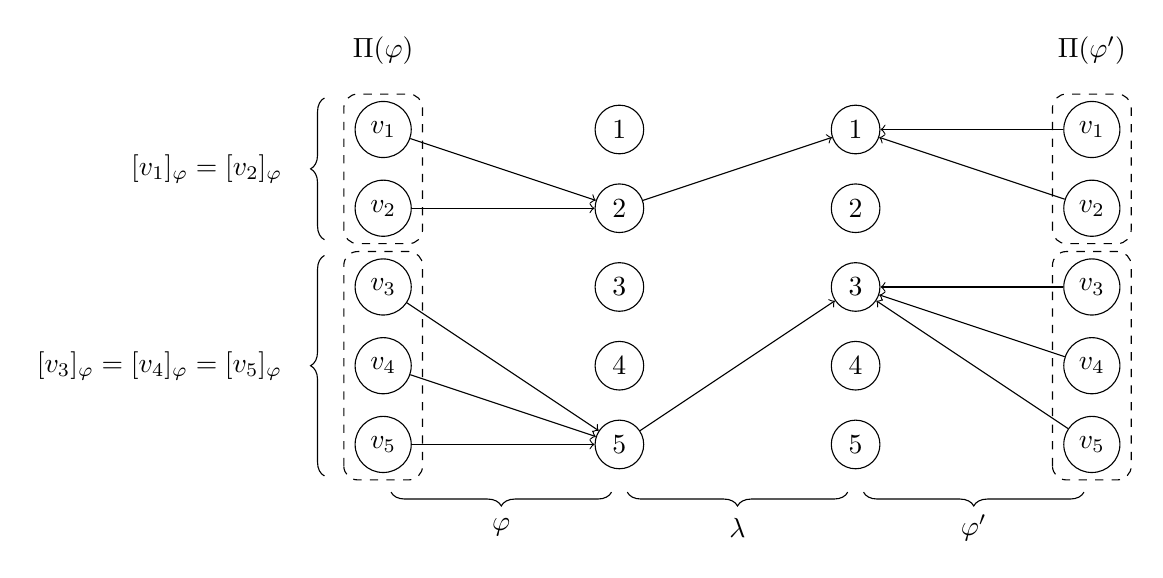
\begin{tikzpicture}
    
    \foreach \s in {1,...,5} {
        \node[draw, circle] (vl\s) at (0,5-\s) {$v_\s$};
        \node[draw, circle] (nl\s) at (3,5-\s) {$\s$};
        \node[draw, circle] (nr\s) at (6,5-\s) {$\s$};
        \node[draw, circle] (vr\s) at (9,5-\s) {$v_\s$};
    }

    \draw[->] (vl1) -- (nl2);
    \draw[->] (vl2) -- (nl2);
    \draw[->] (vl3) -- (nl5);
    \draw[->] (vl4) -- (nl5);
    \draw[->] (vl5) -- (nl5);

    \draw[->] (vr1) -- (nr1);
    \draw[->] (vr2) -- (nr1);
    \draw[->] (vr3) -- (nr3);
    \draw[->] (vr4) -- (nr3);
    \draw[->] (vr5) -- (nr3);

    \draw[->] (nl2) -- (nr1);
    \draw[->] (nl5) -- (nr3);


    \draw [decorate,decoration={brace,amplitude=5pt,mirror,raise=4ex}](0.1,0) -- (2.9,0) node[midway,yshift=-3em]{$\idx$};

    \draw [decorate,decoration={brace,amplitude=5pt,mirror,raise=4ex}](3.1,0) -- (5.9,0) node[midway,yshift=-3em]{$\lambda$};

    \draw [decorate,decoration={brace,amplitude=5pt,mirror,raise=4ex}](6.1,0) -- (8.9,0) node[midway,yshift=-3em]{$\idx'$};

    \node at (0,5) {$\Pi(\idx)$};
    \draw [decorate,decoration={brace,amplitude=5pt,raise=4ex},xshift=-4pt,yshift=0pt](0,-0.4) -- (0,2.4) node [black,midway,xshift=-2.7cm] {$[v_3]_\idx = [v_4]_\idx = [v_5]_\idx$};
    \draw [decorate,decoration={brace,amplitude=5pt,raise=4ex},xshift=-4pt,yshift=0pt](0,2.6) -- (0,4.4) node [black,midway,xshift=-2.1cm] {$[v_1]_\idx = [v_2]_\idx$};
    \draw[rounded corners=5pt, dashed] (-0.5,-0.45) rectangle (0.5,2.45);
    \draw[rounded corners=5pt, dashed] (-0.5,3-0.45) rectangle (0.5,3+1.45);

    \node at (9,5) {$\Pi(\idx')$};
    \draw[rounded corners=5pt, dashed] (9-0.5,-0.45) rectangle (9+0.5,2.45);
    \draw[rounded corners=5pt, dashed] (9-0.5,3-0.45) rectangle (9+0.5,3+1.45);

    \end{tikzpicture}
    \caption{Illustration of two indexings $\idx,\idx'$ with corresponding partitions and proof of equality through part (b) of Theorem \ref{theorem:equal_indexings}.}\label{fig:indexings}
\end{figure}

\begin{definition}
    Let $V = \{ v_1,v_2,\dots, v_n \}$ be a set of $n$ vertices. An indexing of $V$ is a mapping $\idx \in \{ 1,\dots,n \}^V = [n]^V$ that associates every vertex with a number from 1 to $n$.
\end{definition}

\begin{definition}
    Let $\idx$ be an indexing of $V$. The partition induced by $\idx$ is defined as
    \begin{equation}
        \Pi(\idx)= \{ [v]_\idx : v \in V \}, \label{eq:indexing}
    \end{equation}
    where $[v]_\idx = \{ w \in V : \idx(w) = \idx(v) \}$.
\end{definition}

Based on this definition, we are able to obtain some immediate results (proofs in the appendix). First, we are able to use indexings as representations for partitions, i.e. for every partition, there is some indexing that yields that very partition (Lemma \ref{lemma:indexing_partition}). And two, we obtain a criteria that makes it possible to check when two vertices share the same set in the partition (Lemma \ref{lemma:indexing_same_set}).  

\pagebreak 
\begin{lemmarep}
    $\Pi$ is a partition of $V$ if and only if there exists an indexing of $V$ that induces $\Pi$.\label{lemma:indexing_partition}
\end{lemmarep}
\begin{appendixproof}
    First, we will show the direction from left to right. Let $\Pi = \{U_1,\dots,U_m\}$, $1\leq m \leq n$, be a partition of $V$. For all vertices $v$ with corresponding set $U_i$ in $\Pi$ (of which there is exactly one), we define $\idx(v) = i$. For a $j \in \{1,\dots,m\}$ we then obtain $\idx^{-1}(j) = U_j$. But then $\Pi(\idx) = \Pi$, i.e. $\Pi$ is induced by $\idx$. 
    \\
    The other direction requires us to prove that every indexing induces a partition of $V$. I.e., for an indexing $\idx$ of $V$ with $\Pi(\idx)=\Pi$, we need to check the following requirements:
    \begin{enumerate}
        \item $\emptyset \not\in \Pi$:\quad This is obvious from \eqref{eq:indexing}, since every element $[v]_\idx \in \Pi$ contains at least $v$. %https://en.wikipedia.org/wiki/Partition_of_a_set
        \item $\bigcup_{U \in \Pi} U = V$:\quad ``$\subseteq$'' is obvious. For ``$\supseteq$'', take a vertex $v$. Then, $v \in [v]_\idx$ and since $[v]_\idx \in \Pi(\idx)$, we obtain $v \in \bigcup_{U \in \Pi} U$.
        \item if $U_1,U_2 \in \Pi$ and $U_1 \neq U_2$, then $U_1 \cap U_2 = \emptyset$:\quad Take two $U_1, U_2 \in \Pi$ with $U_1 \neq U_2$ such that $U_1 = [w]_\idx$ and $U_2 = [u]_\idx$ for two vertices $w$ and $u$. Assume for a contradiction that $U_1 \cap U_2 \neq \emptyset$, i.e. there exists $v \in U_1 \cap U_2$. But then $v \in [w]_\idx$ and $v \in [u]_\idx$. Thus, $\idx(v) = \idx(w) = \idx(u)$, which cannot be the case, since that would imply $U_1 = U_2$.
    \end{enumerate}
    This completes the proof.
\end{appendixproof}

\begin{lemmarep}
    Let $\idx$ be an indexing of $V$. For all vertices $v,u$, we have $\idx(v) = \idx(u)$ if and only if $v$ and $u$ are part of the same set in $\Pi(\idx)$. \label{lemma:indexing_same_set}
\end{lemmarep}
\begin{appendixproof}
    For the direction from left to right, take $v,u\in V$ such that $\idx(v)=\idx(u)$. Then $v,u \in [v]_\idx = [u]_\idx \in \Pi(\idx)$, i.e. they are part of the same set. For the other direction, we will show the contraposition. Take $v,u\in V$ such that $\idx(v)\neq \idx(u)$. Clearly, $v \in [v]_\idx$ and $v \not\in [u]_\idx$ as well as $u \in [u]_\idx$ and $u \not\in [v]_\idx$. Therefore $[v]_\idx \neq [u]_\idx$. Since by Lemma \ref{lemma:indexing_partition}, $\Pi(\idx)$ is a partition and $[v]_\idx$ and $[u]_\idx$ are distinct sets in $\Pi(\idx)$, $[v]_\idx$ is the only set that contains $v$ and vice versa for $[u]_\idx$ and $u$. Thus, $v$ and $u$ cannot be part of the same set in $\Pi(\idx)$. 
\end{appendixproof}

Since we want to use indexings in order to define transformations on partitions, we are interested in the question when two indexings are ``equal'', in the sense that they induce the same partition. This is characterized in part by Theorem \ref{theorem:equal_indexings}.

\begin{theoremrep}
    If $\idx,\idx'$ are two indexings of $V$, then the following statements are equivalent:
    \begin{enumerate}
        \item[(a)] $\Pi(\idx)=\Pi(\idx')$
        \item[(b)] there is a bijection $\lambda : \image(\idx) \rightarrow \image(\idx')$\footnote{$\image(\idx)$ means the image of $\idx$, i.e. $\image(\idx)=\{ \idx(v) \}_{v \in V}$.} such that $\lambda(\idx(v)) = \idx'(v)$ for all $v \in V$
        \item[(c)] for all vertices $v,w$, $\idx(w) = \idx(v)$ if and only if $\idx'(w) = \idx'(v)$
    \end{enumerate} \label{theorem:equal_indexings}
\end{theoremrep}
\begin{appendixproof}
    We will start with the direction from (a) to (b). Let $\idx$, $\idx'$ be two indexings of $V$ with $\Pi(\idx) = \Pi(\idx')$. We define $\lambda : \image(\idx)\rightarrow \image(\idx')$ as follows. For all $k \in \image(\idx)$, associate a vertex $v$ such that $\idx(v)=k$. Then define $\lambda(k)=\idx'(v)$. It remains to show that $\lambda$ fulfills the requirements in (b):
    \begin{enumerate}
        \item $\lambda$ is bijective:\quad Since every element in $\image(\idx)$ corresponds to a set in $\Pi(\idx)$, and vice versa for $\image(\idx')$ and $\Pi(\idx')$, we get $|\image(\idx)|=|\Pi(\idx)|=|\Pi(\idx')|=|\image(\idx')|$. Since $\image(\idx)$ and $\image(\idx')$ are also finite, it suffices to show injectivity of $\lambda$ in order to prove bijectivity. Assume for a contradiction that $\lambda$ is not injective, i.e. there are $v_1,v_2 \in V, \idx(v_1) \neq \idx(v_2)$, such that $\lambda(\idx(v_1))=\lambda(\idx(v_2))=\idx'(v_1)=\idx'(v_2)$. Thus, by application of Lemma \ref{lemma:indexing_same_set}, there must be a set in $\Pi(\idx')$ that contains $v_1$ and $v_2$, while there is no set in $\Pi(\idx)$ that has both vertices in it. But then $\Pi(\idx)\neq \Pi(\idx')$. Contradiction.
        \item For all vertices $v$, $\lambda(\idx(v)) = \idx'(v)$: \quad Take an arbitrary vertex $v$ and let $\idx(v) = k \in \image(\idx)$. Let $\bar{v}$ be the vertex that was previously associated with $k$ in the definition of $\lambda$, i.e. the vertex for which $\idx(\bar{v})=k = \idx(v)$ and $\lambda(\idx(\bar{v}))=\idx'(\bar{v})$ holds. Assume for a contradiction that $\idx'(v)\neq \idx'(\bar{v})$. By Lemma \ref{lemma:indexing_same_set}, this yields that there is no set in $\Pi(\idx')$ that contains both $v$ and $\bar{v}$, while there is one in $\Pi(\idx)$. But then again $\Pi(\idx) \neq \Pi(\idx')$, i.e. a contradiction. Thus, $\lambda(\idx(v)) = \lambda(\idx(\bar{v})) = \idx'(\bar{v}) = \idx'(v)$. 
    \end{enumerate}
    This concludes this direction. For the direction from (b) to (c), let $\lambda$ be a bijection between the images of two indexings $\idx, \idx'$ of $V$ that fulfills the requirements in (b). Let $w,v$ be two arbitrary vertices; then
    \begin{align*}
        \idx(w) = \idx(v) &\quad\text{iff}\quad \lambda(\idx(w)) = \lambda(\idx(v)) &(*) \\ 
        &\quad\text{iff}\quad \idx'(w) = \idx'(v) &(**)
    \end{align*}
    The first identity $(*)$ works since $\lambda$ is a bijection and the second $(**)$ since $\lambda(\idx(w))=\idx'(w)$ for all vertices $w$.
    The remainder (c) to (a) is relatively trivial: If we assume premise (c), then
    \begin{align*}
        U \in \Pi(\idx) &\quad\text{iff}\quad U = [v]_\idx \text{ for a vertex $v$} \\
        &\quad\text{iff}\quad U = \{ w \in V : \idx(w) = \idx(v) \} \text{ for a vertex $v$} \\
        &\quad\text{iff}\quad U = \{ w \in V : \idx'(w) = \idx'(v) \} \text{ for a vertex $v$} \\ 
        &\quad\text{iff}\quad U = [v]_{\idx'} \text{ for a vertex $v$} \\
        &\quad\text{iff}\quad U \in \Pi(\idx'),
    \end{align*}
    which shows $\Pi(\idx)=\Pi(\idx')$.
\end{appendixproof}

If the task is to determine whether two induced partitions $\Pi(\idx)$, $\Pi(\idx')$ for given indexings $\idx,\idx'$ of $V$ are equal, the result of Theorem \ref{theorem:equal_indexings} might be useful: instead of explicitly computing the resulting partitions and checking if both sets are equal, one can simply determine whether a fitting bijection $\lambda$ exists, which is arguably easier. In fact, one can construct $\lambda$ as in the first part of the proof of Lemma \ref{theorem:equal_indexings} and then check whether the result is a bijection or not. Figure \ref{fig:indexings} illustrates two indexings, their partitions and some of the findings of Theorem \ref{theorem:equal_indexings}.


\section{Move-Operation on Indexings}

We will now define the ``move''-operation on indexings, which transforms an indexing into another indexing by changing the assigned index of a vertex. The effect this has on the induced partition is that the respective vertex is ``taken'' from its original set\footnote{i.e. the set $[v]_\idx$} and then ``put into'' some other set\footnote{i.e. the set $\idx^{-1}(k)$, where $k$ is some number between $1$ and $n$}. This is then defined as $\move: [n]^V \times V \times [n] \rightarrow [n]^V$ with 
\begin{equation} 
\move(\idx, v, k)(u) = \begin{cases}
    \idx(u) & u \neq v, \\ 
    k & u = v
\end{cases} \label{eq:move-operation}
\end{equation} 
for every vertex $u$. The operation takes as input an indexing $\idx$, a vertex $v$ and new index $k$ and outputs a new indexing that is essentially the same as $\idx$, with the only difference being that $v$ is mapped to $k$ instead of whatever it was mapped to before.
\\ \\
In many cases, there are multiple ways of moving one vertex to different indices while still inducing the same partition afterwards. For example, if $v$ is an arbitrary vertex, $\idx$ is an indexing of $V$ with $\idx^{-1}(k_1) = \dots = \idx^{-1}(k_m) = \emptyset$ and $k_1,\dots,k_m$ are pairwise different, then moving $v$ to $k_1,\dots,k_m$ yields that while $\move(\idx,v,k_1),\dots,\move(\idx,v,k_m)$ are all different indexings, their induced partitions are the same: $\Pi(\move(\idx,v,k_1)) = \dots = \Pi(\move(\idx,v,k_m))$.
\\ 
Based on this observation we are interested in an efficient way of enumerating all possible ``moves'' of a vertex with respect to the induced partitions without enumerating too much or having to double-check whether two move-operations induce the same partition. Hence, consider algorithm \ref{alg:1}, which aims at finding a solution to this problem.

\begin{algorithm}[H]
    \SetAlgoLined
    \KwIn{Set of vertices $V$ with indexing $\idx$}
    \KwResult{Sequence of indexings $\idx_1,\idx_2,\dots,\idx_m$ }
    Let $<$ be some linear order on $V$ \;
    Let $\mathcal{N} := \{1,\dots,n\}\backslash \image(\idx)$ \;
    \ForAll{vertices $w \in V$}{
        \ForAll{$\idx(v) \in \image(\idx) \backslash \{ \idx(w) \}$}{
            \uIf{$[w]_\idx = \{ w, u, \dots \}$ or $[v]_\idx  = \{ v, s, \dots \}$}{
                enumerate $\move(\idx,w,\idx(v))$ \;
            }\uElseIf{$[w]_\idx = \{ w \}$ and $[v]_\idx = \{ v \}$ and $w < v$}{
                enumerate $\move(\idx,w,\idx(v))$ \;
            }
        }
        \uIf{$[w]_\idx = \{ w, u, v, \dots \}$ or $([w]_\idx = \{w,u\}$ and $w < u)$}{
            Let $k \in \mathcal{N}$ \;
            enumerate $\move(\idx,w,k)$ \;
        }
    }
    \caption{Move-Enumeration} \label{alg:1}
\end{algorithm}

We want to check three important properties: one, algorithm \ref{alg:1} only enumerates indexings which yield partitions distinct from all induced partitions of the other indexings (the ``not too much''-part, see Lemma \ref{lemma:pairwise_distinctiveness}), two, every partition that is induced when moving one vertex in $\idx$ to a different set is induced by some indexing in $\idx_1,\dots,\idx_m$ (Lemma \ref{lemma:completeness}) and three, the partition that is induced by $\move(\idx,v,k)$ for any vertex $v$ and number $k$ is not the same that is induced by $\idx$ (Lemma \ref{lemma:self_neighbour}).

%A corollary of these properties would be that there is a bijection between the sets $ \{\idx_1,\dots,\idx_m\}$ and $\{ \Pi(\move(\idx,v,k)) : v \in V, k \in \{1,\dots,n\} \}\backslash \{ \Pi(\idx) \}$.

\begin{lemmarep}[Pairwise Distinctiveness]
    Let $\idx$ be an indexing of $V$ and $\idx_1,\dots,\idx_m$ be a sequence generated by algorithm \ref{alg:1} on input $V$ and $\idx$. Then for all pairwise distinct $i,j \in \{1,\dots,m\}$, we have $\Pi(\idx_i) \neq \Pi(\idx_j)$. \label{lemma:pairwise_distinctiveness}
\end{lemmarep}
\begin{appendixproof}
    First note that $\idx_1,\dots,\idx_m$ are indeed results of a move-operation on $\idx$. This can be checked by simple introspection on algorithm \ref{alg:1}. Therefore, we can write $\idx_i = \move(\idx,w_i,k_i)$ for all $i=1,\dots,m$, with $w_i \in V$ and $k_i \in \{1,\dots,n\}$, i.e.: $\idx_i$ moves vertex $w_i$ to index $k_i$. \\
    % By Lemma \ref{lemma:equal_indexings}, we conclude that there must be a bijection $\lambda : \image(\idx_i) \rightarrow \image(\idx_j)$ such that for all vertices $v$, $\lambda(\idx_i(v)) = \idx_j(v)$.
    Secondly, note that every pair $(w,k) \in V \times \{1,\dots,n\}$ is regarded at most once. This means that for every two different indexings $\idx_i,\idx_j$, either $w_i \neq w_j$ or $k_i \neq k_j$ holds. Now, pick $i,j \in \{1,\dots,m\}$ such that $i \neq j$. The rest of the proof can be done via case distinction on all possible conditions under which a move-operation could be executed in the algorithm:
    \begin{enumerate}
        \item $w_i = w_j = w$. Since $i$ and $j$ are pairwise distinct, $k_i \neq k_j$ must hold. For $k_i$, we have either $k_i \in \mathcal{N}$ (line 10) or $k_i = \idx(v) \in \image(\idx)\backslash \{ \idx(w) \}$ (line 6 and 8):
        \begin{enumerate}
            \item If $k_i \in \mathcal{N}$: Then $\idx_i(w) = k_i$ only for $w$ (since there is no vertex that is mapped to $k_i$ in $\idx$). Also $k_j \not\in \mathcal{N}$, since there is at maximum one $k \in \mathcal{N}$ for which $\move(\idx,w,k)$ is enumerated. Thus, $k_j = \idx(v) \in \image(\idx)\backslash \{ \idx(w) \}$. But then we have $\idx_j(w) = k_j =\idx_j(v)$ and $\idx_i(v) = k_j \neq k_i = \idx_i(w)$, which implies $\Pi(\idx_i) \neq \Pi(\idx_j)$ by Theorem \ref{theorem:equal_indexings}.
            \item If $k_i = \idx(v) \in \image(\idx)\backslash \{\idx(w) \}$: After moving $w$ to $k_i$ in $\idx_i$, one obtains $\idx_i(w) = \idx_i(v) = k_i$, and after moving $w$ to $k_j$ in $\idx_j$, one gets $\idx_j(w) = k_j \neq k_i = \idx_j(v)$. But that implies $\Pi(\idx_i) \neq \Pi(\idx_j)$ by Theorem \ref{theorem:equal_indexings}.  
        \end{enumerate}
        \item $w_i \neq w_j$, and therefore $\idx_i(w_j) = \idx(w_j)$ and $\idx_j(w_i) = \idx(w_i)$ (i.e., $\idx_i$ does not change the index of $w_j$ and $\idx_j$ does not change the index of $w_i$). Again, we make the distinction for the case $k_i \in \mathcal{N}$ and $k_i = \idx(v) \in \image(\idx)\backslash \{ \idx(w) \}$:
        \begin{enumerate}
            \item If $k_i \in \mathcal{N}$: since $k_i \not\in \image(\idx)$, $\idx(w_i) \neq k_i$. Also, at least one of the following cases (see line 9 of the algorithm) must hold:
            \begin{enumerate}
                \item If $[w_i]_\idx = \{ w_i, u, v, \dots \}$: At least one of the vertices $u$ and $v$ must be different from $w_j$, since $u \neq v$ and $w_j$ cannot be equal to both of them. Let w.l.o.g. $u \neq w_j$. Then $\idx_j(w_i) = \idx(w_i) = \idx(u) = \idx_j(u)$ but $\idx_i(w_i) = k_i \neq \idx(w_i) = \idx_i(u)$, i.e. $\Pi(\idx_i) \neq \Pi(\idx_j)$ by Theorem \ref{theorem:equal_indexings}.
                \item If $[w_i]_\idx = \{w_i, u \}$ and $w_i < u$: 
                \begin{enumerate}
                    \item $w_j \neq u$: We get $\idx_i(w_i) \neq \idx_i(u)$ and $\idx_j(w_i) = \idx(w_i) = \idx(u) = \idx_j(u)$. Then simply apply Theorem \ref{theorem:equal_indexings} and obtain $\Pi(\idx_i) \neq \Pi(\idx_j)$.
                    \item $w_j = u$. Since $u \not< w_i$ and $[w_j]_\idx = [w_i]_\idx$, there is no possibility that line 11 is executed for $w_j$. Therefore, $k_j \not\in \mathcal{N}$. But then $k_j= \idx(v) \in \image(\idx)\backslash \{ \idx(w_j) \}$ with $w_i \neq v \neq w_j$. Thus, $\idx_j(w_j) = \idx(v)=\idx_j(v)$ and $\idx_i(w_j) = \idx(w_j) \neq \idx(v) = \idx_i(v)$. Again, the application of Theorem \ref{theorem:equal_indexings} yields $\Pi(\idx_i) \neq \Pi(\idx_j)$.
                \end{enumerate}
            \end{enumerate}
            \item If $k_i = \idx(v) \in \image(\idx)\backslash \{ \idx(w_i) \}$, then one of the following cases applies:
            \begin{enumerate}
                \item $[w_i]_\idx = \{w_i,u,\dots\}$. 
                \begin{enumerate}
                    \item If $w_j = u$: then $\idx_j(w_i) = \idx(w_i) \neq \idx(v) = \idx_j(v)$ and $\idx_i(w_i) = \idx(v) = \idx_i(v)$. Here, Theorem \ref{theorem:equal_indexings} can be applied, which results in $\Pi(\idx_i) \neq \Pi(\idx_j)$.
                    \item If $w_j \neq u$: then $\idx_j(w_i) = \idx(w_i) = \idx(u) = \idx_j(u)$ and $\idx_i(w_i) \neq \idx(w_i) = \idx(u) = \idx_i(u)$. Theorem \ref{theorem:equal_indexings} can be applied with result $\Pi(\idx_i) \neq \Pi(\idx_j)$.
                \end{enumerate}
                \item $[v]_{\idx} = \{v,s,\dots\}$.
                \begin{enumerate}
                    \item If $w_j = v$: then $\idx_i(w_i) = \idx_i(v)$ but $\idx_j(w_i) \neq \idx_j(v)$ . In this case, Theorem \ref{theorem:equal_indexings} can be applied to obtain $\Pi(\idx_i) \neq \Pi(\idx_j)$.
                    \item If $w_j \neq v$: then $\idx_i(w_i) = \idx_i(v)$ but $\idx_j(w_i) \neq \idx_j(v)$. Application of Theorem \ref{theorem:equal_indexings} yields $\Pi(\idx_i) \neq \Pi(\idx_j)$.
                \end{enumerate}
                \item $[w_i]_\idx = \{ w_i \}$ and $[v]_\idx = \{ v \}$ and $w_i < v$.
                \begin{enumerate}
                    \item If $w_j = v$. Then neither line 6 (since $|[w_j]_\idx| = 1$) nor line 8 are executed for $w_j$ and $k = \idx(w_i)$ (since $w_j \not < w_i$). Thus, $k_j \neq \idx(w_i)$ must hold. But then $\idx_i(w_i) = k_i = \idx(v) = \idx(w_j) = \idx_i(w_j)$ and $\idx_j(w_i) = \idx(w_i) \neq k_j = \idx_j(w_j)$. Application of Theorem \ref{theorem:equal_indexings} yields $\Pi(\idx_i) \neq \Pi(\idx_j)$.
                    \item If $w_j \neq v$. Then $\idx_i(w_i) = \idx(v) = \idx_i(v)$ but $\idx_j(w_i) = \idx(w_i) \neq \idx(v) = \idx_j(v)$. Again, application of Theorem \ref{theorem:equal_indexings} gives us $\Pi(\idx_i) \neq \Pi(\idx')$.
                \end{enumerate} 
            \end{enumerate}
        \end{enumerate}
    \end{enumerate}
    This finishes the proof, since in all cases $\Pi(\idx_i) \neq \Pi(\idx_j)$ holds.
\end{appendixproof}

\begin{lemmarep}[Completeness]
    Let $\idx$ be an indexing of $V$ and $\idx_1,\dots,\idx_m$ be the sequence that is generated by algorithm \ref{alg:1} on input $V$ and $\idx$. For all vertices $v$ and $k \in \{1,\dots,n\}$ such that $\Pi(\move(\idx,v,k)) \neq \Pi(\idx)$, there is $i\in \{1,\dots,m\}$ such that $\Pi(\move(\idx,v,k)) = \Pi(\idx_i)$.\label{lemma:completeness}
\end{lemmarep}
\begin{appendixproof}
    Let $\idx$ be an indexing of $V$ and let $w$ be a vertex and $k\in\{1,\dots,n\}$. We want to show that if $\Pi(\move(\idx,w,k)) \neq \Pi(\idx)$, then there is an $i\in \{1,\dots,m\}$ such that $\Pi(\move(\idx,w,k)) = \Pi(\idx_i)$. First, note that $\idx(w)\neq k$ holds, since otherwise this would imply $\Pi(\move(\idx,w,k)) = \Pi(\idx)$. The remainder of this proof works with multiple case distinctions:
    \begin{enumerate}
        \item If $[w]_\idx = \{ w \}$. This directly implies $k = \idx(v)$ for a $v \in V$, since otherwise that would mean $\Pi(\move(\idx,w,k)) = \Pi(\idx)$. Thus, for $[v]_\idx$ there are the following options:
        \begin{enumerate}
            \item If $[v]_\idx = \{ v \}$. In the case $w < v$, line 8 enumerates $\move(\idx,w,k)$ directly.  Otherwise, if $v < w$, line 8 enumerates $\move(\idx,v,\idx(w))$, where $\Pi(\move(\idx,v,\idx(w)) = \Pi(\move(\idx,w,k))$. 
            \item If $[v]_\idx = \{ v,s,\dots \}$. Line 6 in the algorithm directly enumerates $\move(\idx,w,k)$.
        \end{enumerate} 
        \item If $[w]_\idx = \{ w,u, \dots \}$. Since $\idx$ maps $w$ and $u$ to the same index, there is at least one index in $1,\dots,n$ that is assigned no vertex. But then $\mathcal{N} \neq \emptyset$. Again, there are the following options:
        \begin{enumerate}
            \item There is no $v \in V$ such that $k = \idx(v)$: 
            \begin{enumerate}
                \item If $[w]_\idx = \{ w,v,u,\dots \}$, then line 11 is executed and there is some $\ell \in \mathcal{N}$ for which $\move(\idx,w,\ell)$ is enumerated. But then $\Pi(\move(\idx,w,k))=\Pi(\move(\idx,w,\ell))$.
                \item If $[w]_\idx = \{w,u\}$. 
                \begin{enumerate}
                    \item If $w < u$, then line 11 enumerates $\move(\idx,w,\ell)$ for $w$ and some $\ell \in \mathcal{N}$. But then $\Pi(\move(\idx,w,\ell)) = \Pi(\move(\idx,w,k))$.
                    \item If $u < w$, then line 11 enumerates $\move(\idx,u,\ell)$ for $u$ and some $\ell \in \mathcal{N}$. But then again, $\Pi(\move(\idx,u,\ell)) = \Pi(\move(\idx,w,k))$.
                \end{enumerate} 
            \end{enumerate}
            \item There is $v \in V$ such that $k = \idx(v)$. Then $k \in \image(\idx)\backslash \{ \idx(w) \}$ and line 6 is executed. This enumerates $\move(\idx,w,k)$.
        \end{enumerate}
    \end{enumerate}
    This shows that in all cases, there is some $\idx_i$ that is enumerated which yields the same partition as $\move(\idx,v,k)$.
\end{appendixproof}

\begin{lemmarep}
    Let $\idx$ be an indexing of $V$ and $\idx_1,\dots,\idx_m$ be the sequence that is generated by algorithm \ref{alg:1} on input $V$ and $\idx$. Then $\Pi(\idx) \neq \Pi(\idx_i)$ for all $i\in \{1,\dots,m\}$. \label{lemma:self_neighbour}
\end{lemmarep}
\begin{appendixproof}
    $\Pi(\move(\idx,v,k)) = \Pi(\idx)$ if and only if either $k=\idx(v)$ or if $[v]_\idx = \{v\}$, then $k \in \mathcal{N}$. Simple case distinction yields that both cases never happen for any $\idx_i$, $i\in \{1,\dots,m\}$.
\end{appendixproof}

\begin{corollary}
    For an indexing $\psi$ of $V$, the following statements are equivalent:
    \begin{itemize}
        \item $\psi = \move(\idx,v,k)$ and $\Pi(\psi)\neq \Pi(\idx)$ for $v \in V, 1\leq k \leq n$
        \item $\Pi(\psi) \in \{\Pi(\idx_1),\dots,\Pi(\idx_m)\}$.
    \end{itemize}
\end{corollary}
\begin{proof}
    From top to bottom, simply apply Lemma \ref{lemma:completeness}. For the direction from bottom to top, apply Lemma \ref{lemma:self_neighbour}.
\end{proof}


%\bibliography{column_generation}{}
%\bibliographystyle{plain}

\end{document}